\documentclass{llncs}

\usepackage[latin1]{inputenc}
\usepackage{graphicx}        % standard LaTeX graphics tool
\usepackage{url}
\usepackage{listings}
\usepackage{subfig}
%\usepackage{apalike}

\begin{document}

\title{A statistical approach to dealing with noisy fitness in evolutionary algorithms}
% Zeineb - A statistical approach to deal with noisy fitness in evolutionary algorithms
% Zeineb - A statistical approach dealing with noisy fitness in evolutionary algorithms
% Thanks, Zeineb - JJ

\author{J.J. Merelo, Zeineb Chelly, Antonio
  Mora, Antonio Fern\'andez-Ares, Anna
  I. Esparcia-Alc\'azar, Carlos Cotta, Paloma de las Cuevas, Nuria
  Rico}
\institute{University of Granada, 
       Department of Computer Architecture and Technology, ETSIIT, and CITIC \url{http://citic.ugr.es}
       18071 - Granada, Spain \\ 
       Laboratoire de Recherche Op\'erationelle de D\'ecision et de Contr\^ole de Processus, Institut Sup\'erieur de Gestion, Tunisia.\\
Universidad de M\'alaga,
Departamento de Lenguajes y Ciencias de la Computaci\'on, M\'alaga, Spain\\ %CARLOS: affiliation corrected
Universidad de Granada; Depto. Estad\'istica e Investigaci\'on Operativa, Granada, Spain
\email{\{jmerelo,pedro,amorag,antares\}@geneura.ugr.es,palomacuevasd@gmail.com,
  zeinebchelly@yahoo.fr, aiesparcia@gmail.com,
ccottap@lcc.uma.es,nrico@ugr.es,}
}

\maketitle

\begin{abstract}
In most computer games as in life, the outcome of a match is uncertain due
  to several reasons: the characters or assets appear in different initial
  positions or the response of the player, even if programmed, is not
  deterministic; different matches will yield different scores. That is a
  problem when optimizing a game-playing engine: its fitness will be
  noisy, and if we use an evolutionary algorithm it will have to deal
  with it. This is not straightforward since there is an inherent
uncertainty in the true value of the fitness of an individual, or
rather whether one chromosome is better than another, thus making it preferable for selection.
Several methods based on implicit or explicit average or
changes in the selection of individuals for the next generation have been proposed in the past, 
but they involve a substantial redesign of the algorithm and the
software used to solve the problem. In this paper we propose  new
methods based on incremental computation (memory-based) or fitness average or, additionally, using
statistical tests to impose a partial order on the population; this
partial order is considered to assign a fitness value to every individual
which can be used straightforwardly in any selection function. 
Tests using several
hard combinatorial optimization problems show that, despite
an increased computation time with respect to the other methods, both memory-based methods have a higher
success rate than {\em implicit} averaging methods that do not use
memory; however, there is not a clear advantage in success rate or
algorithmic terms of one method over the other. 

\end{abstract}

\keywords{Evolutionary algorithms, noisy optimization problems,
  dynamic problems}
%--------------------------------------------------------------------------

\section{Introduction}
In our research on the optimization of the behavior of bots or game
strategies, we have frequently found that the fitness of a bot is {\em
  noisy}, in the sense that repeated evaluations will yield different
values \cite{DBLP:journals/jcst/MoraFGGF12} which is a problem since
fitness is the measure used to select individuals for reproduction. If
we look at it in a more general setting, 
% Zeineb - If we look at it in a more general setting, ... ("it" not
% "in")
% Corrected, thx, - JJ
noise in the fitness of individuals in the context of an evolutionary algorithm has different origins. It can be inherent to the
individual that is evaluated; for instance, in 
\cite{DBLP:journals/jcst/MoraFGGF12} a game-playing bot (autonomous agent) that includes a set of application rates is optimized. This results in different
actions in different runs, and obviously different success rates and
then fitness. Even comparisons with other individuals can be affected:
given exactly the same pair of individuals, the chance of one beating
the other can vary in a wide range. In other cases like the one
presented in the MADE environment, where whole worlds are evolved
\cite{2014arXiv1403.3084G} the same kind of noisy environment will
happen.  When using evolutionary algorithms to optimize stochastic
methods such as neural networks \cite{castilloGECCO99}
using evolutionary algorithms the measure that is usually taken as
fitness, the success rate, will also be noisy since different training
schedules will result in slightly different success rates. 

The examples mentioned above are actually included in one of the four categories
% Paloma - [...] actually included in [...] || [...] in one (or in |
% of) the four [...]
% fixed, thanks - JJ
where uncertainties in fitness are found, fitness functions with intrinsic noise. These four types include also,
according to \cite{Jin2005303} approximated fitness functions
(originated by, for instance, surrogate models); robust functions,
where the main focus lies on finding values with high tolerance to
% [...] where the main focus lies on [...]
% fixed, thx - JJ
change in initial evaluation conditions, and finally dynamic fitness
functions, where the {\em inherent} value of the function changes with
time. 
Our main interest will be in the first type, since it is the one
that we have actually met in the past and has led to the development
% Paloma - This line works fine without 'which' because it is already
% implied.
% out - JJ
of this work. 

At any rate, in this paper we will not be dealing with actual
problems; we will try to simulate the effect of noise by adding to the fitness function Gaussian noise centered in 0 and $\sigma=1,2,4$. We will deal mainly with combinatorial optimization functions with noise added having the same shape and amplitude,
that we actually have found in problems so far. In fact, from the
point of view of dealing with fitness, these are the main features of
noise we will be interested in. 

This paper is an extension of \cite{merelo14:noisy}. The main problem
found in those set of experiments was the amount of evaluations needed
to find a solution to the problem; while an individual was in the
population, it was re-evaluated (re-sampled). However, statistically a
limited amount of evaluations is usually enough to make meaningful,
and statistically significant, comparisons. That is why in this paper
we have done two kind of improvements: improve speed, because
implementation always matters
\cite{DBLP:conf/iwann/MereloRACML11},
and limit the amount of evaluations while checking if the results
achieved (mainly success rate) remain the same.  

The rest of the paper is structured as follows: in the next section we describe the
% Paloma - I would personally use 'structured as follows', but it is up to you. And probably after the colon you
% should start with 'in the next chapter/section [...]' just to
% clarify.
% done - JJ
state of the art in the treatment of noise in fitness functions. The
method we propose in this paper, called Wilcoxon Tournament, will be
shown in Section \ref{sec:wilcoxon}; experiments are described and
results shown in Section \ref{sec:res}; finally its implications are discussed in the last section of the paper. 

%--------------------------------------------------------------------------

\section{State of the art}
\label{sec:soa}

\sloppypar The most comprehensive review of the state of the art in evolutionary
algorithms in {\em uncertain} environments 
was done by %Jin and Branke in 2005 -- CARLOS: inline reference; no need to add authors in text
\cite{Jin2005303}, although recent
papers such as \cite{DBLP:journals/corr/QianYZ13,6931307} and \cite{Qian:sampling} include a brief update of the state
of the art. In that first survey 
of evolutionary optimization by Jin and Branke  in
uncertain environments that uncertainty is categorized into noise,
robustness, fitness approximation and time-varying fitness functions, and then,
different options for dealing with it are proposed. In principle, the
approach presented in this paper was designed to deal with the first kind of
uncertainty, noise in fitness evaluation, although it could be argued
that there is uncertainty in the true fitness as stated in the third
category. In any case it could be applied to
other types of noise, since it depends more on the shape and intensity
of noise than the origin. 

\sloppypar In the same situation, a noisy fitness evaluation, several solutions have been
proposed and explained in the survey \cite{Jin2005303}. These will be
explained next.
% Zeineb - In this situation, several solutions have been proposed
% ... ("have" not "were")
% fixed, thx - JJ
For scientists not concerned on solving the problem of noise, but on
a straightforward solution of the optimization problem without
modification of existing tools and methodologies, a usual approach is
just to disregard the fact that the fitness is 
noisy and use whatever value is returned by a single evaluation or after
re-evaluation each generation. 
% Zeineb - A usual approach is just to disregard the fact that the fitness is noisy and 
%to use whatever value is returned a single time or after a
%re-evaluation of each generation.
% fixed, thx - JJ
This was the option in our
%CARLOS: references split in order to avoid margin problems
previous research in games \cite{bots:evostar,DBLP:journals/jcst/MoraFGGF12,Liberatore_COSECIVI14} and evolution of neural networks \cite{castilloGECCO99,merelo:ESNN} and leads, if
the population is large enough, to an {\em implicit averaging} as
mentioned in \cite{Jin2005303}. In fact, selection used in evolutionary algorithms
is also stochastic, so noise in fitness evaluation
will have the same effect as randomness in selection or a higher mutation
rate, which might make the evolution process easier and not harder
in some particular cases
\cite{DBLP:journals/corr/QianYZ13}. 
In fact, Miller and Goldberg proved that an infinite population would not
be affected by noise \cite{miller1996genetic} and Jun-Hua and Ming studied the
effect of noise in convergence rates \cite{Junhua20136780}, proving
that an elitist genetic algorithm finds at least one solution, although with a lowered
convergence rate. But real populations are finite, so the usual
approach to dealing with fitness with a degree of randomness is to
increase the population size to a value bigger than 
would be needed in a non-noisy environment. In fact, it has been
recently proved that using {\em sex}, that is, crossover, is able to
deal successfully with noise \cite{2015arXiv150202793F}, while an
evolutionary algorithm based on mutation
%CARLOS: un algorithm mu+1 puede usar cruce - elimino esto  (such as the $\mu$+1 EA)
would suffer a considerable degradation of performance. 
% Zeineb - (such as the $\mu$+1 EA) would suffer from a considerable degradation in terms of performance.
However, crossover is part of the standard kit of evolutionary
algorithms, so using it and increasing the population size has the
advantage that no special provision or change to the implementation
has to be made, just different values of the standard parameters.

Another more theoretically sound way is using a statistical central tendency
indicator, which is usually the {\em average}. This strategy is called
{\em explicit averaging} by Jin and Branke and is used, for instance,
in 
\cite{Junhua20136780}. Averaging decreases the variance of fitness but
the problem is that it is not clear in advance what would be the
sample size used for averaging \cite{aizawa1994scheduling}. Most
authors use several measures of fitness for each new individual
\cite{costa2013using}, although other averaging strategies have also
been proposed, like averaging over the neighbourhood of the
individual or using {\em resampling}, that is, more measures of fitness in a
number which is decided heuristically
\cite{liu2014mathematically}. This assumes that there is, effectively,
an average of the 
fitness values which is true for Gaussian random noise and other
distributions such as Gamma or Cauchy but not
necessarily for all distributions. 
To the best of our knowledge, 
other measures like the median which might be more adequate for
certain noise models have not been tested; the median always exists,
while the average might not exist for non-centrally distributed
variables. Besides, most models keep the number of evaluations fixed 
and independent of its value, 
% Zeineb - Besides, most models keep the number of evaluations   fixed
% and independent of its value, 
% fixed, thx- JJ
which might result in bad individuals
being evaluated many times before being discarded; some authors have
proposed {\em resampling}, that is, re-evaluate the individuals a number of times to increase the precision in fitness
\cite{RadaVilela2014,6900521}, 
which will effectively increase the number of
evaluations and thus slow down the search. In any case, using average is
also a small change to the overall algorithm framework, requiring only
using as new fitness function the average of several evaluations.
We will try to address this in the model presented in this
paper. 

These two approaches that are focused on the evaluation process might
be complemented with changes to the selection process. For instance,
using a threshold \cite{Rudolph2001318,6900521} that is related to the noise characteristics to
avoid making comparisons of individuals that might, in fact, be very
similar or statistically the same; this is usually called {\em
  threshold selection} and can be applied either to explicit or
implicit averaging fitness functions. The algorithms used for
solution, themselves, can be also tested, with some authors proposing, instead of taking more measures, 
testing different solvers \cite{cauwet2014algorithm}, some of which
might be more affected by noise than others. However, recent papers
have proved that sampling might be ineffective \cite{Qian:sampling} in
some types of evolutionary algorithms, adding running time without an
additional benefit in terms of performance. This is one lead we will
use in the current paper. 

Any of these approaches do have the problem of statistical
representation of the {\em true} fitness, even more so if there is not
such a thing, but several measures that represent, {\em as a set}
the fitness of an individual. This is what we are going to use in this
paper, where we present a method that uses resampling via an
individual memory and use either explicit averaging or statistical
tests like the non-parametric Wilcoxon test. 
First we will examine and try to find the shape of the noise that
actually appears in games; then we will check in this paper what is the influence on the quality of
results of these two strategies and which one, if any, is the best
when working in noisy environments.  

%--------------------------------------------------------------------------

\section{Noise in games: An analysis}
\label{sec:noise}

In order to measure the nature of noise, we are going to use the data
that is available to us, fitness evaluations in the
Planet Wars game, that has been used as a framework for evolving strategies, e.g., \cite{DBLP:journals/jcst/MoraFGGF12}, and other game contents, e.g., \cite{lara2014balance}. %CARLOS: reference added
In this game when one player {\em invades} a planet the outcome depends
deterministically on the number of {\em ships} each player has; however, players are positioned randomly with the
constraint that they should be far enough from each other; other than
that, any planet in the game can be an initial position. The planetary
map is also random, chosen from 100 possibilities. Besides, in
the strategy used in that game by our bot \cite{DBLP:conf/iwann/Fernandez-AresMMGF11}, actions are not deterministic, since
every player is defined by a set of probabilities to take one course
of action. 

In order to have enough measures to model the noise, an evolutionary algorithm with standard parameters was run with the
main objective of measuring the behavior of fitness. A sample of ten
individuals from generation 1 and another 10 from generation 50 were
extracted. The fitness of each individual was measured 100 times. 
The main intention was also to see how noise evolved with
time. Intuitively we thought that, since the players become better
with evolution, the noise and thus the standard deviation would
decrease. However, what we found is shown in Figure \ref{fig:sd},
which shows a plot of the standard deviation in both generations and
illustrates the fact that the spread of fitness values is {\em bigger}
as the evolution proceeds, going from around 0.15 to around 0.20. 
%
\begin{figure}[ht!b]
\centering
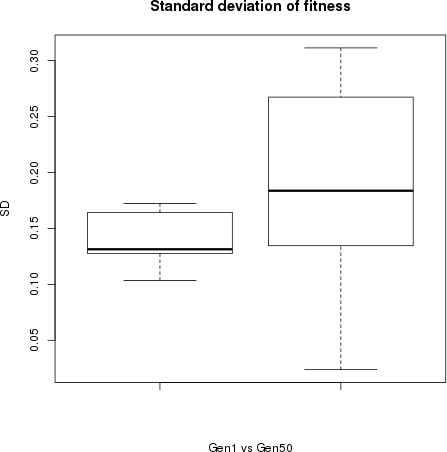
\includegraphics[width=0.8\textwidth]{../images/sd.png}
\caption{Boxplot of standard deviation of noise fitted to a normal
  distribution, left for the first generation and right for the
  50th. Fitness averages around 1. \label{fig:sd}}
\end{figure}
%
This result might be a bit misleading since the average values of
the fitness increase at the same time, but it implies that the noise
level might be around 20\% of the {\em signal} in these kind of problems. 

By taking these measures, we were also interested in checking whether, in fact, the normal
distribution is the best fit for the fitness measures, thus making
averages of fitness appropriate for modeling the whole set of fitness
measures. We tested three
distributions: Gamma, Weibull and normal (Gaussian) distribution after
doing an initial test that included (and discarded) Cauchy and Exponential. All this
analysis was done using the library {\tt fitrdist} in R, and data as
well as scripts needed to do it are publicly available in the GitHub repository. After trying
to fit these three distribution to data in generation 1 and 50, we
analyzed goodness-of-fit using the same package and the {\tt gofstat}
function. This function yields several measures of goodness, including
the Akaike Information Criterion and the Kolmogorov-Smirnov statistic.

What we found was that, in all cases, Gamma is the distribution that
better fits the data. That does not mean that the noise effectively
follows this distribution, but that it is, of all distributions, the
one that best fits the data. In fact, just a few individuals have a good fit (to
% Paloma - better use "it is" than "it's"
% done, but you can change this if you want by yourself - JJ
95\% accuracy using the Kolmogorov-Smirnov), and none of them in
generation 50. The fit for an individual in the first generation that
does follow that distribution (individual 8) is shown in Figure
\ref{fig:indi8}. The main difference between Gamma and Gaussian is
that Gamma is skewed, instead of being centered about a particular
value. 
%
\begin{figure}[!t] %CARLOS: place figure at top of page
\centering
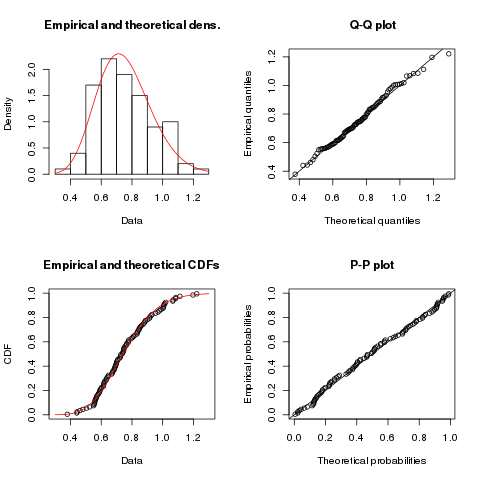
\includegraphics[width=0.95\textwidth]{../images/indi8.png}
\caption{Fit of the fitness value of an individual in the first
  generation of the evolutionary algorithm to a gamma distribution,
  showing an histogram in the top left corner, CDFs in the bottom left
  corner and quantile-quantile and percentile-percentile plots in the
  right hand side. \label{fig:indi8}}
\end{figure}

This figure also shows that, even if it is skewed, its skewness is not
too high which makes it close to the standard distribution (which is
considered a good
approximation if $k>10$). However, it is interesting to note the
% Zeineb ($k >$ 10) the > character was not displayed for me, butit's ok in your generated .pdf 
% then no need to take this comment into consideration
%CARLOS: punt mathematical symbols inside the math env to avoid encoding problems.
skewness inherent in the distribution as a feature of noise, at least
in this particular game. 

Some interesting facts that can be deduced from these measures is that
in general, fitness is skewed and its standard deviation has a high
value, up to 20\% in some cases. Besides, it
follows a gamma distribution, which, if we want to model noise
% Paloma - "if we want to model noise"
% argh, thx - JJ
accurately, should be the one used. However, we are rather interested
in the overall shape of noise so since the skewness parameter of the gamma
distribution is rather high we will use, in this paper, a Gaussian
noise to simulate it; Gaussian is a good approximation of Gamma for
high values of the skewness parameter. This will be used in the experiments shown
below. 
% Zeineb - This will be used in the experiments discussed in Section \ref{sec:res}.
% Zeineb - by "below" you mean in Section \ref{sec:res}? or both Section \ref{sec:res} and Section \ref{sec:wilcoxon} ?
% Zeineb - beacuse experiments are in Section \ref{sec:res} ...


\section{Fitness memory and statistical significant differences}
\label{sec:wilcoxon}

As indicated in previous section, 
% Zeineb - As indicated in the previous section, 
most explicit averaging methods
use several measures to compute fitness as an average, with
resampling, that is, additional measures, in case 
comparisons are not
statistically significant. In this paper we will introduce a fitness
{\em memory}, which amounts 
to a resampling every generation an
individual survives. An individual is born with a fitness
memory of a single value, with memory size increasing with {\em
  survival} time. This is actually a combination of an implicit and an 
explicit evaluation strategy: {\em younger} individuals are rejected
outright if their fitness computed after a single evaluation is not
enough to participate in the pool, while  {\em older} ones use several
measures to compute average fitness, which means that averages will be
a more precise representation of actual value. 
As evolution proceeds,
the best individuals will, effectively, have an underlying non-noisy
best value. We will call this method {\em extended temporal average}
or {\sf ETA}. 
% Zeineb - We will call this method {\em Extended Temporal Average} or {\sf ETA}. 
However, since average is a single value, selection methods might, in
fact, select as the best individuals some that are not if the comparison
is not statistically significant; this will happen mainly in the first
and middle stages of search, which might effectively eliminate from
the pool 
%  Zeineb - which might be effectively eliminated from the pool 
% Zeineb - (not sure if I have understoof the meaning) Check it if it's correct or not, please.
or not adequately represent individuals that constitute, in
fact, good solutions. That is why we introduce an additional feature:
using Wilcoxon test \cite{wilcoxon:1945}
for comparing not the average, but all
fitness values attached to an individual. This second method
introduces a partial order in the population pool: two individuals
might be different (one better than the other) or not \cite{wilcoxon:ga}. There are many
possible ways of introducing this partial order in the evolutionary
algorithm; however, what we have done is to pair individuals a certain
number of times (10, by default) and have every individual score a
point every time it is better than the other in the couple; its score
will be decreased by one if it is the worse one. An individual that is better
% Paloma - "it will be deducted by one point" sounds better than "it
% will get a point less", which sounds like '+= -1'
% changed - JJ
that all its couples will have a fitness of 20; one whose comparisons
are never significant according to the Wilcoxon test will score
exactly 10, the same as if it wins as many times as it loses, and the
one that always loses will score 0. We will call this method
Wilcoxon-test based partial order, or {\sf WPO} for short.
% Zeineb - We will call this method Wilcoxon-test based on Partial Order, or {\sf WPO} for short.
\begin{figure}[!t] %CARLOS: place figure at top of page
\centering
\subfloat[Memory size]{
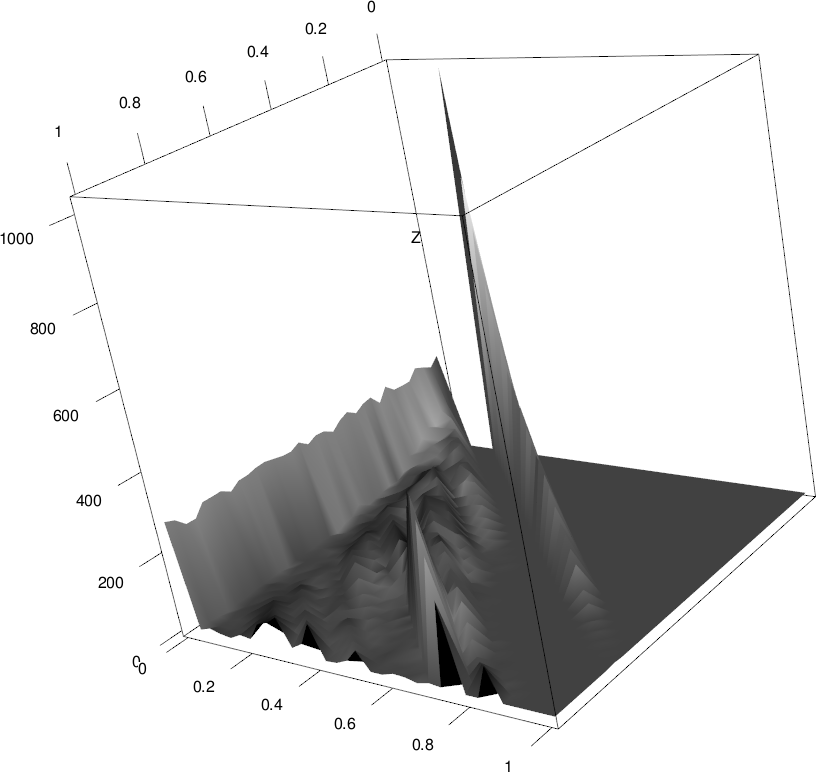
\includegraphics[width=0.5\textwidth]{../images/memory-size.png}
}
~
\subfloat[Fitness distribution]{
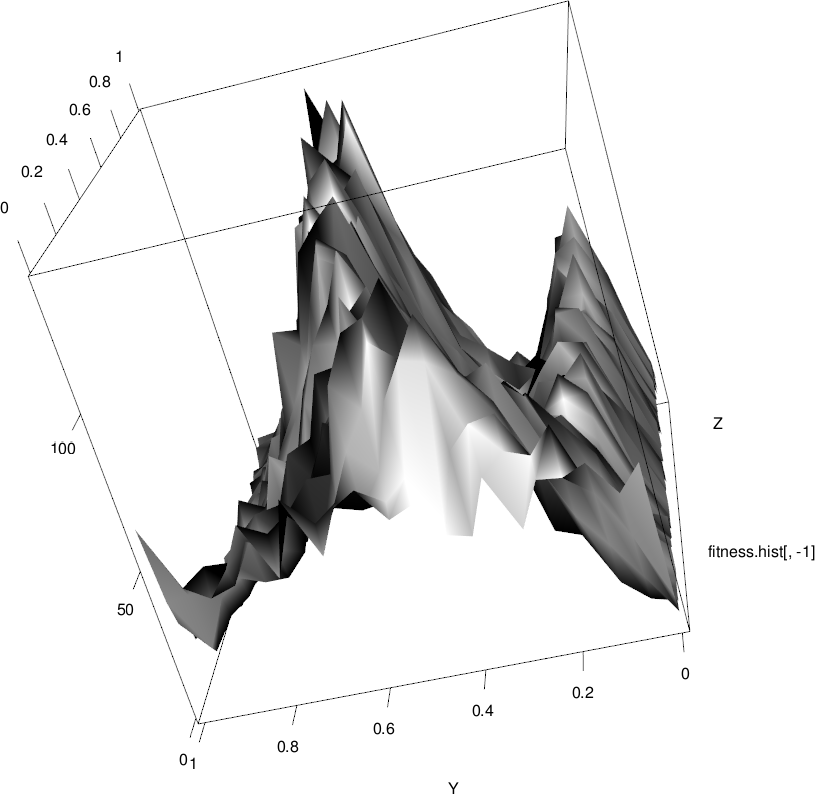
\includegraphics[width=0.5\textwidth]{../images/fitness-distribution.png}
}
\caption{(Left) 3D plot of the distribution of memory sizes for a single
execution of the Wilcoxon-test based partial order. (Right)
3D plot of the distribution of fitness values along time for the WPO
% Paloma - Capital d on 3D
% OK - JJ
method on the Trap function. \label{fig:initial}}
\end{figure}

\sloppypar Initial tests, programmed in Perl using {\tt
  Algorithm::Evolutionary} \cite{ae09} (available with an open %CARLOS: edit to avoid alignment problems
  %CARLOS: URLS as footnotes. They disrupt the flow of the text and are more clearly accessible at the bottom of the page
source license\footnote{\url{http://git.io/a-e}}) were made with these two types of algorithms and the
Trap function \cite{wilcoxon:ga}, showing the best results for the WPO
method and both of them being better that
the implicit average method that uses a single evaluation per
individual, although they needed more time and memory. Since it does not need to perform averages or make
additional fitness measures every generation, it is twice as fast as
the next method, the one that uses explicit average fitness. An
exploration of memory sizes\footnote{\url{http://jj.github.io/Algorithm-Evolutionary/graphs/memory/} } %(published in
% Zeineb - (published at
(shown in Figure \ref{fig:initial} for a
typical run) showed that they are distributed unevenly but, in general, there is no single memory size
overcoming all the population. Besides, distribution of fitness\footnote{\url{http://jj.github.io/Algorithm-Evolutionary/graphs/fitness-histo/}} shows a
distribution with most values concentrated along the middle (that is,
fitness equal to 10 or individuals that cannot be compared with any
other,
% % Zeineb - fitness equals to 10 or individuals
 together with a few with the highest fitness and many with the
lowest fitness. Besides showing that using the partial order for individual selection 
is a valid strategy, it also shows that a too greedy selection method would
eliminate many individuals that might, in fact, have a high fitness. This
will be taken into account when assigning parameter values to the
evolutionary algorithm that will be presented next.


%--------------------------------------------------------------------------

\section{Results}
\label{sec:res}

ETA and WPO have been tested using two well-known benchmarks, the deceptive bimodal Trap \cite{deb1992analyzing}
function and the Massively Multimodal Deceptive Problem \cite{goldberg92massive} (MMDP). 
We chose to use just these two functions 
% Paloma - 'were chosen' is redundant.
% OK - JJ
because they have different fitness landscapes, are usually difficult
for an evolutionary algorithm and have been extensively used for
testing other kind of operators and algorithms.

Several methods were tested: a baseline algorithm without
noise to establish the time and number of evaluations
needed to find the solution, a 0-memory (implicit average) method that
uses noisy fitness without making any special arrangement, ETA and
WPO. Evolutionary algorithm parameters and code for all tests were the
same, except in one
particular case: we used 2-tournament with 50\% replacement, 20\%
mutation and 80\% crossover, $p=1024$ and stopping when the best was
found or number of evaluations reached. This was 200K for the Trap,
which used 40 as chromosome size, and 1M for MMDP, which used 60 as
chromosome size; these parameters are shown in Table \ref{fig:ga_params}. We have also used an additive Gaussian noise centered in zero
and different $\sigma$, which is independent of the range of variation of the fitness values. By default, noise will follow a normal distribution with center in 0 and $\sigma=1$.

\begin{table*}[!t]%CARLOS: places table at the top of the page.
\begin{center}
\caption{Common evolutionary algorithm parameters}
\label{fig:ga_params}
\begin{tabular}{lc}%{p{3cm}p{7cm}}
\hline\noalign{\smallskip}
\noalign{\smallskip}
Parameter & Value \\
\hline
\noalign{\smallskip}
Chromosome length & 40 (Trap) 60 (MMDP)\\
Population size & 1024\\
Selection & 2 tournament selection \\
Replacement rate & 50\% \\
Mutation rate & 20\% \\
Crossover rate &  80\% \\
Max evaluations & 200K (Trap) 1 Million(MMDP) \\
Stopping criterion & Non-noisy best found or maximum number of  evaluations reached \\
\hline
\end{tabular}
\end{center}
\end{table*}



\begin{figure}[!t] %CARLOS: place figure at top of page
\centering
\subfloat[Memory size]{
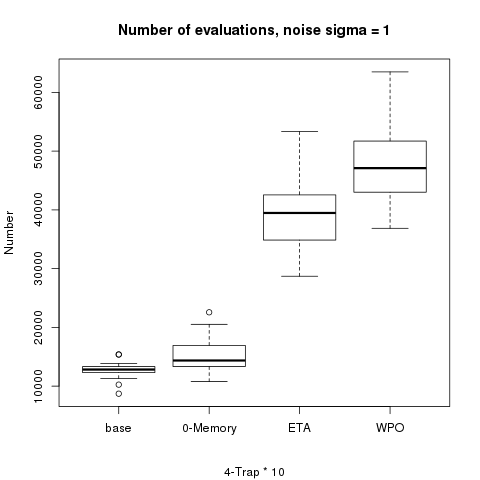
\includegraphics[width=0.45\textwidth]{../images/trap-evals-all.png}
}
~
\subfloat[Fitness distribution]{
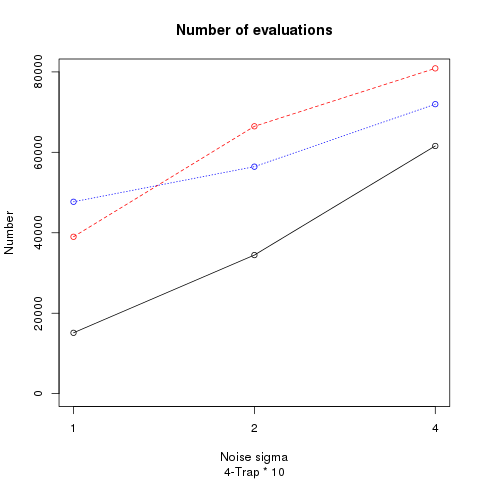
\includegraphics[width=0.45\textwidth]{../images/trap-noisy-evals.png}
}
\caption{(Left) Comparison of number of evaluations for the 4-Trap x
  10 function and the rest of the algorithms with a noise $\sigma$
  equal to 1. (Right). Plot of average number of evaluations for
  different methods: 0 memory (black, solid), ETA (red, dashed), WPO
  (blue, dot-dashed). \label{fig:trap:evals}}
\end{figure}
%
All tests use the {\tt Algorithm::Evolutionary} library, and the scripts
are published, as above, in the GitHub repository, together with raw
and processed results. The evolutionary algorithm code used in all
cases is exactly the same except for WPO, which, since it needs the
whole population to evaluate fitness, needed a special reproduction
and replacement library. This also means that the replacement method
is not exactly the same: while WPO replaces every generation 50\% of
the individuals, the rest evaluate new individuals before replacement
and eliminate the worst 512 (50\% of the original
population). 
% Zeineb - the rest evaluates new individuals before replacement and eliminates the 
Replacement is, thus, less greedy in the WPO case, but
we do not think this will be a big influence on result 
% Zeineb - but we do not think that this will have a big influence on the results
(although it might account for the bigger number of evaluations obtained in some
cases), besides, it just needed a small modification of code and was
thus preferred for that reason. All values shown are the result of 30
independent runs.

The results for different noise levels are shown in Figure
\ref{fig:trap:evals}. The boxplot on the left hand side compares the
number of evaluations for the baseline method and the three methods
with  $\sigma=1$. The implicit average method (labelled as 0-memory) is
only slightly worse than the baseline value of around 12K evaluations,
with the ETA and WPO methods yielding very similar values which are
actually worse than the 0-memory method. However, the scenario on the
right,
 which shows how the number of evaluations scales with the noise
level, is somewhat different. 
% is somehow different. 
While the 0-memory method still has the
smallest number of evaluations {\em for successful runs}, the success
rate degrades very fast, with roughly the same and slightly less than
100\% for $\sigma=2$ but falling down to 63\% for 0-memory and around
80\% for ETA and WPO (86\% and 80\%). That is, best success rate is
shown by the ETA method, but the best number of evaluations for
roughly the same method is achieved by WPO. 

These results also show that performance degrades quickly with problem
difficulty and the degree of noise, that is why we discarded the
0-memory method due to its high degree of failure (a high percentage of the runs did not find the solution) with noise = 10\%
max fitness and evaluated ETA and WPO over another problem, MMDP with
similar absolute $\sigma$, with the difference that, in this case,
$\sigma=2$ would be 20\% of the max value, which is close to the one
observed experimentally, as explained in the Section \ref{sec:noise}.
% Zeienb - in  Section \ref{sec:noise}.
\begin{figure}[!t] %CARLOS: place figure at top of page
\centering
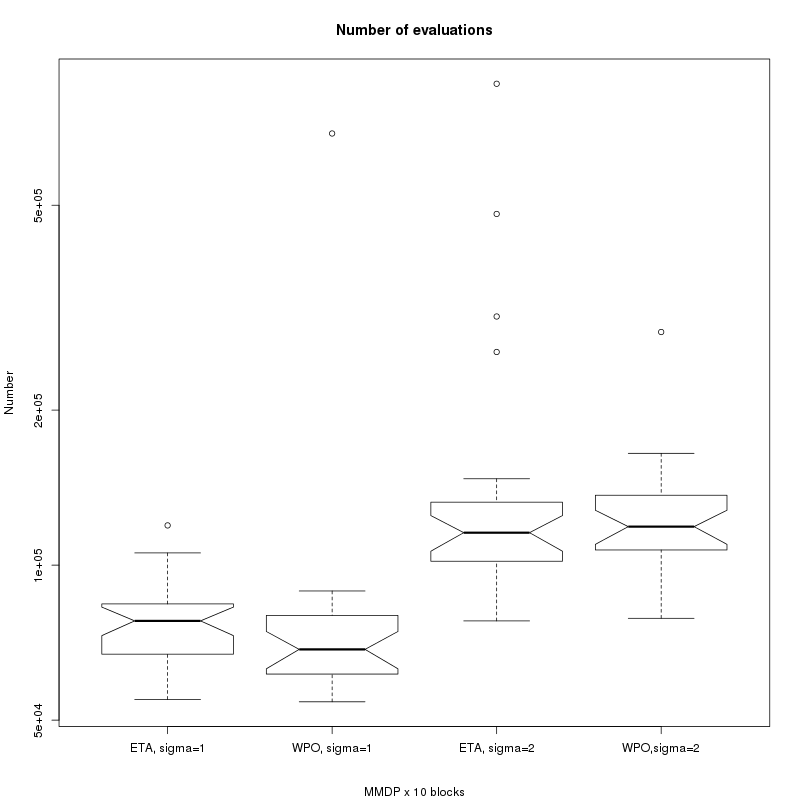
\includegraphics[width=0.9\textwidth]{../images/evals-mmdp.png}
\caption{Number of evaluations for successful runs ETA and WPO needed for solving the MMDP
  problem with 10 blocks and different noise levels, $\sigma=1,2$. \label{fig:mmdp:evals}}
\end{figure}
%
The evolutionary algorithm for MMDP used exactly the same parameters
as for the Trap function above, except the max number of evaluations, which
was boosted to one million. Initial tests with the 0-memory method
yielded a very low degree of success, which left only the two methods
analyzed in this paper for testing with MMDP. 
Success level was in all cases around 90\% and very similar in all experiments; the number of evaluations is more affected by noise and shown in
Figure \ref{fig:mmdp:evals}. 
In fact, WPO and ETA have a very similar
number of evaluations. It is statistically indistinguishable for
$\sigma=2$, and different only at the 10\% level (p-value = 0.09668)
for $\sigma=1$, however, if we take the time needed to reach solutions
into account, ETA is much faster since it does not apply 10*1024
statistical tests every generation. 
% zeineb - statistical tests in every generation. 
However, WPO is more robust, with
a lower standard deviation, in general, at least for high noise
levels. However, both methods obtain a good result with a much higher
% Zeineb - both methods obtain  good results with a much higher
success rate than the implicit fitness (0-memory) method. Besides, ETA and WPO 
incorporate explicit fitness evaluation naturally into the population
{\em resampling} only surviving individuals. This accounts for a
predictable behavior of the algorithm, since the number of evaluations
per generation is exactly the population size, which is important for
optimization processes with a limited budget. 

%--------------------------------------------------------------------------

\section{Conclusions}

In this paper we have introduced two methods to deal with the problem
of noisy fitness functions. The two methods, {\sf ETA}, based on
re-evaluation of surviving individuals and {\sf WPO}, which uses the
Wilcoxon test to compare a sample of individuals and partial-order
them within the population, 
 have been tested over two
different fitness functions and compared with implicit average (or
0-memory) methods, as well as among themselves. In general,
memory-based methods have much higher success rate than 0-memory
methods and the difference increases with the noise level, with
0-memory methods crashing at noise levels close to 20\% while ETA and
WPO maintain a high success level.

It is difficult to choose between the two proposed methods, ETA and
WPO. However, ETA is much faster since it avoids costly
comparisons. It also has a slightly higher success rate, and the
number of evaluations it needs to find the solution is only slightly
worse; even if from the point of view of the evolutionary algorithm it
is slightly less robust and slightly worse, it compensates the time
needed to make more evaluations with the fact that it does not need to
perform statistical tests to select new individuals.

However, this research is in initial stages. 
% Zeineb - However, this research is in its initial stages. 
The fact that we are
using a centrally distributed noise gives ETA an advantage since, in
fact, comparing the mean of two individuals will be essentially the
same as doing a statistical comparison, since when the number of
measures is enough, statistical significance will be reached. In fact,
with a small difference ETA might select as better an individual whose
fitness is actually the same, something that would be correctly
spotted by WPO, but, in fact, since there is an average selective
pressure this is not going to matter in the long run. 

It might matter in different situations, for instance in numerical
optimization problems and also when noise follows an uniform
distribution; behavior might in this case be similar to when noise
levels are higher. These are scenarios that are left for future
research, and destined to find out in which situations WPO is better
than ETA and the other way round. 

Besides exploring noise in different problems and modelling its
distribution, we will explore different parameters. The first one is the number of comparisons in WPO. Initial
explorations have proved that changing it from 5 to 32 does not yield
a significant difference. Looking for a way to speed up this method
would also be important since it would make its performance closer to
ETA. Memory size could also be explored. Right now evaluations are
always performed, but in fact after a number of evaluations are done
comparisons will be statistically significant; it is difficult to
know, however, which is this number, but in long runs it would be
interesting to cap fitness memory size to a sensible number, or, in
any case, see the effect of doing it. 

\section*{Acknowledgments} %CARLOS: makes unnumbered section and adds project reference.

This work has been supported in part by project EphemeCH
(TIN2014-56494-C4-3-P and TIN2014-56494-C4-1-P) and DNEMESIS (P10-TIC-6083).
The authors would like to thank the FEDER of European Union for
financial support via project ``Sistema de Informaci\'on y Predicci\'on de
bajo coste y aut\'onomo para conocer el Estado de las Carreteras en
tiempo real mediante dispositivos distribuidos" (SIPEsCa) of the
"Programa Operativo FEDER de Andaluc\'ia 2007-2013". We also thank all
Agency of Public Works of Andalusia Regional Government staff and
researchers for their dedication and professionalism.

Our research group is committed to Open Science and the writing and
development of this paper has been carried out in GitHub at this
address \url{https://github.com/JJ/noisy-fitness-eas}. We encourage you
to visit, comment and to do all kind of suggestions or feature
requests.

We would like also to thank Marc Schoenauer for the suggestion that
has been put to test in this paper.


\begin{figure}[!h]
\begin{center}

\includegraphics[width=10cm]{../images/logos_SIPESCA_2.jpg}
\end{center}
\end{figure}

\bibliographystyle{apalike}
\bibliography{geneura,wilcoxon}  

\end{document}
